\chapter[Results and discussion]{Results and discussion}

\section{Results}

This section presents calculation results, such as the effective multiplication 
factor for whole core, neutron flux spectrum, temperature reactivity 
coefficients, and compares the results against those obtained by Park \emph{et al.} using Monte Carlo \gls{MCNP}6 \cite{park_whole_2015}. 

Figure~\ref{fig:park_detailed_view} illustrates Park \emph{et al.} model which ignores lengthwise graphite ridges at each corner of each graphite element in zone I, II-A, and significantly simplifies in zone II-B and annulus. The normalized neutron flux distribution is calculated for the whole core using continuous-energy nuclear data. The temperature coefficients for both fuel salt solution and reactor graphite are computed by comparing effective multiplication factors for two temperatures in the working range.

\begin{figure}[htp!] % replace 't' with 'b' to 
  \centering
  \vspace{-0.3em}
  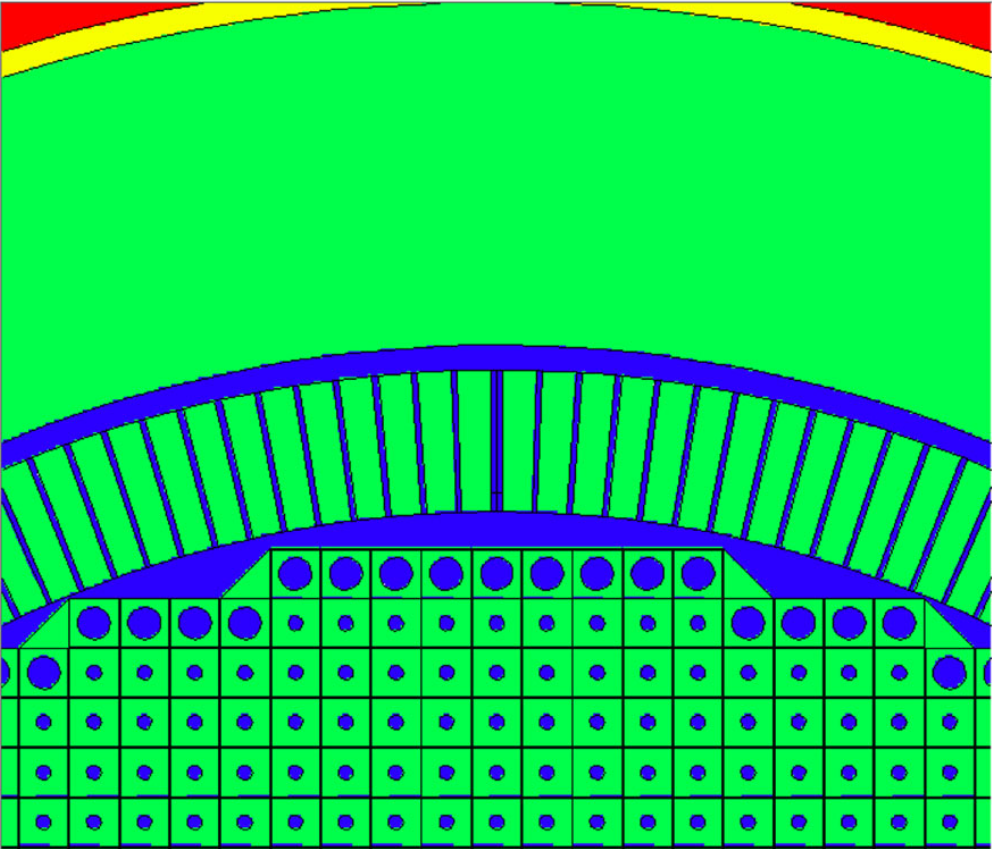
\includegraphics[width=0.9\textwidth]{park_detailed_view.png}
  \caption{Detailed plan view of Park (MCNP6) model \cite{park_whole_2015}.}
  \vspace{-0.6em}
  \label{fig:park_detailed_view}
\end{figure}
 	
\subsection{Neutron spectrum}
Fig.~\ref{fig:spectrum} demonstrates the normalized neutron flux spectrum for 
the whole core in the energy range from $10^{-9}$ to $10$ MeV. The results show 
close fit with the MCNP simulation \cite{park_whole_2015}, especially in 
thermal energy range.  
\begin{figure}[t!] % replace 't' with 'b' to force it to 
  \centering
  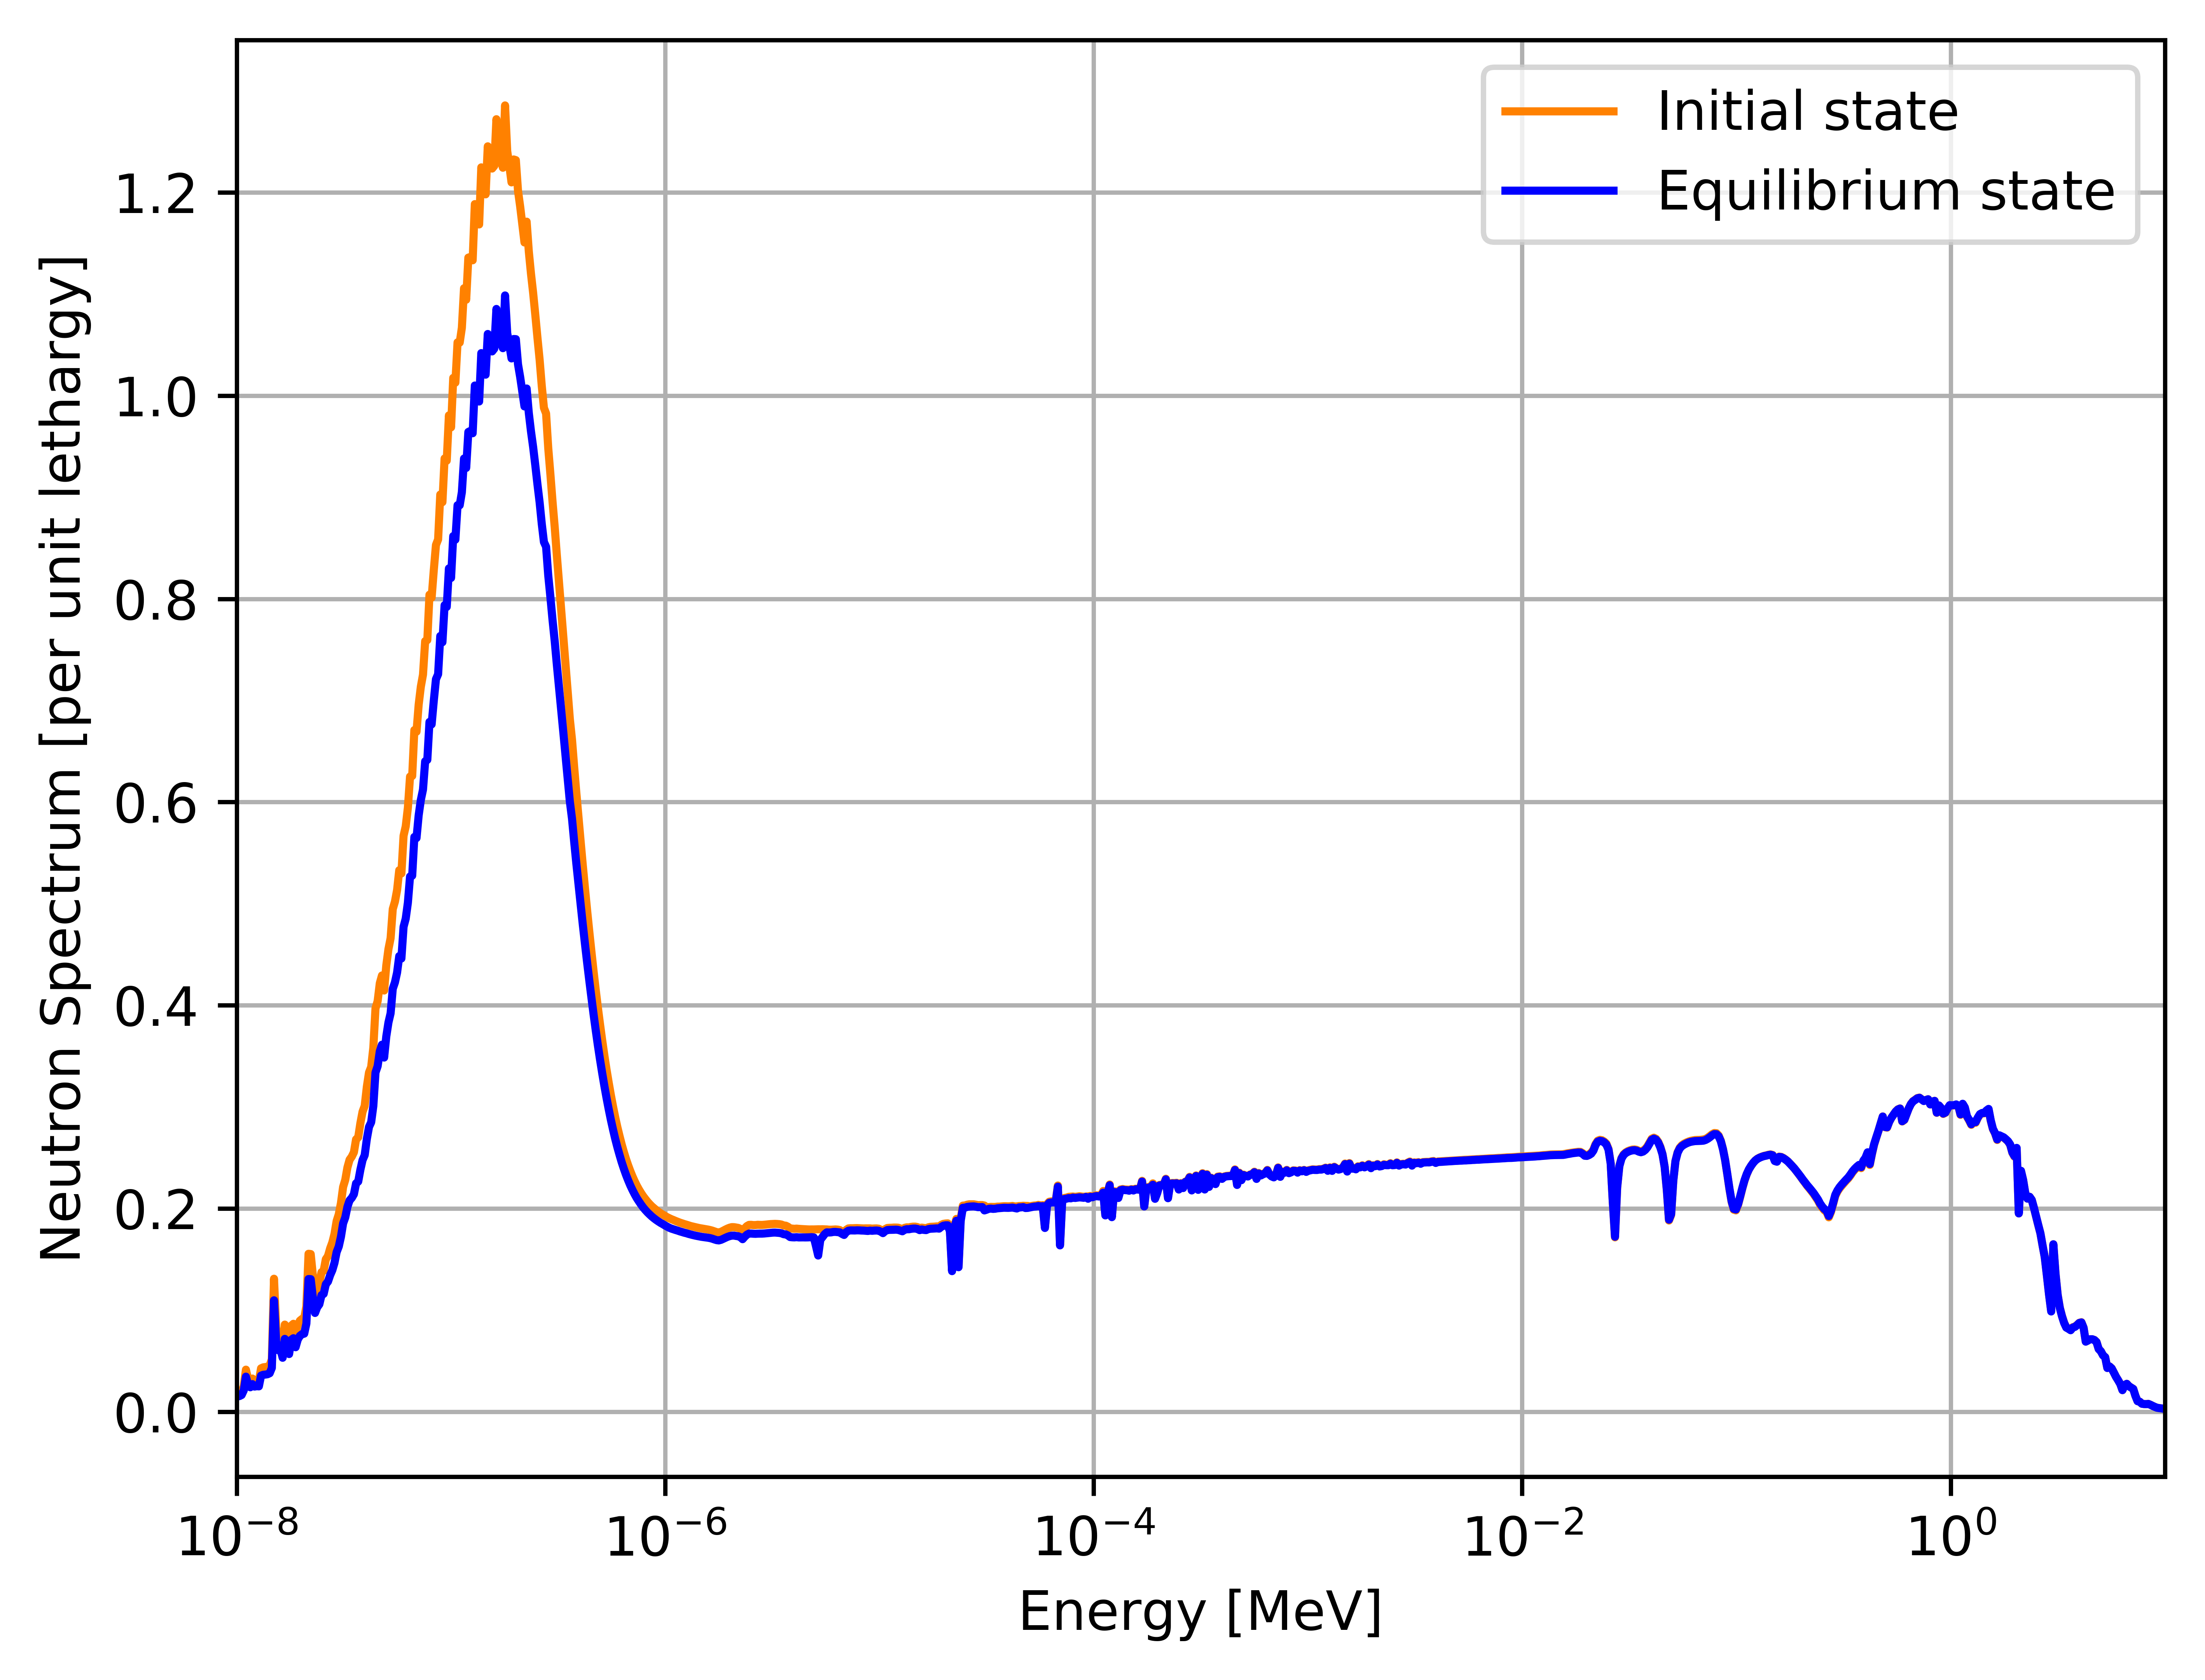
\includegraphics[width=1.05\linewidth]{spectrum.png} \caption{Neutron flux 
  spectrum of \gls{MSBR} for MCNP6 and SERPENT model.}
  \label{fig:spectrum}
\end{figure}
It is important to obtain the epithermal and thermal spectrum to produce 
$^{233}$U from $^{232}$Th because radiative capture cross section of thorium 
monotonically decreases from $10^{-10}$ MeV to $10^{-5}$ MeV. Hardening the 
spectrum tends to significantly increase resonance absorption in thorium and 
decrease the absorptions in fissile and construction materials. Thus, a 
signficant amount fissile material will be needed to make the reactor critical.

\subsection{Effective multiplication factor}
Table~\ref{tab:keff} shows the effective multiplication factor for both MCNP6 
and Serpent 2 whole core models. The factor obtained using Serpent 2 is 300 pcm 
lower than that obtained by Park \emph{et al.} using MCNP6 
\cite{park_whole_2015}. Standard deviations are 5 and 9 pcm, respectively. The 
discrepancy is likely due to simplificiations to the Zone II geometry model 
used in Park \emph{et al.}
%%%%%%%%%%%%%%%%%%%%%%%%%%%%%%%%%%%%%%%%
\captionsetup[table]{
  labelsep = newline,
  name = TABLE, justification=justified,
  singlelinecheck=false,%%%%%%% a single line is centered by default
  labelsep=colon,%%%%%%
  skip = \medskipamount}
\begin{table}[h!]
%\centering
\caption{Effective multiplication factor of whole core model.}
\begin{tabular}{p{0.15\linewidth} p{0.3\linewidth} p{0.3\linewidth}} \toprule
      & Serpent2      & MCNP6 \cite{park_whole_2015}          \\ \midrule
K$_{eff}$  & 1.00389$\pm$0.00005 & 1.00736$\pm$0.00009
\\
\bottomrule
\end{tabular}
  \label{tab:keff}
\end{table}
%%%%%%%%%%%%%%%%%%%%%%%%%%%%%%%%%%%%%%%%%%%%%%%%%%%%%%%%%%%%%%%%%%%%%%%%%%%%%%%%
\subsection{Temperature effect of reactivity}
Table~\ref{tab:tcoef} shows temperature effects on reactivity calculated in 
this work as compared to both \cite{park_whole_2015} and 
\cite{robertson_conceptual_1971}. Uncertainty for each temperature coefficient 
also appears in Table~\ref{tab:tcoef}. The main physical principle underlying 
the reactor temperature feedback is an expansion of matter when it is heated.  
When the fuel salt temperature increases, the density of the salt decreases, 
but at the same time, the total volume of fuel salt in the core remains 
constant because it is bounded by the graphite. When the reactor graphite 
temperature grows, the density of graphite declines creating additional space 
for fuel salt. To determine temperature coefficients, the cross-section 
temperatures for fuel and moderator were changed from 900K to 1200K. Three 
different cases were considered:
\begin{enumerate}  \item Temperature of fuel salt rising from 900K to 1200K.
\item Temperature of graphite rising from 900K to 1200K.  \item Whole reactor 
        temperature rising from 900K to 1200K.
\end{enumerate}

%%%%%%%%%%%%%%%%%%%%%%%%%%%%%%%%%%%%%%%%
\captionsetup[table]{
  labelsep = newline,
  name = TABLE, justification=justified,
  singlelinecheck=false,%%%%%%% a single line is centered by default
  labelsep=colon,%%%%%%
  skip = \medskipamount}
\begin{table}[h!]
%\centering
  \caption{Temperature coefficients of reactivity.}
\begin{tabular}{p{0.22\linewidth} p{0.22\linewidth} p{0.21\linewidth} 
        p{0.15\linewidth}} \toprule
   Reactivity coefficient [pcm/K]  & Serpent2      & MCNP6 
        \cite{park_whole_2015}   & Reference \cite{robertson_conceptual_1971}      
        \\ \midrule
Fuel salt        & $-3.70\pm0.016$ & $-3.20\pm0.05$ & $-3.22$ \\ \midrule
Moderator        & $+2.33\pm0.027$ & $-0.11\pm0.05$ & $+2.35$ \\ \midrule
Total            & $-1.57\pm0.033$ & $-3.21\pm0.04$ & $-0.87$ \\
\bottomrule
\end{tabular}
  \label{tab:tcoef}
\end{table}
%%%%%%%%%%%%%%%%%%%%%%%%%%%%%%%%%%%%%%%%%%%%%%%%%%%%%%%%%%%%%%%%%%%%%%%%%%%%%%%%
In the first case, changes in the fuel temperature only impact fuel density. In 
this case, the geometry is unchanged because fuel is a liquid. However, when 
the moderator heats up, both the density and the geometry change due to thermal 
expansion of the solid graphite blocks and reflector. Accordingly, the new 
graphite density was calculated using a linear temperature expansion 
coefficient of 1.3$\times10^{-6}$1/K \cite{robertson_conceptual_1971}. A new 
geometry input was created based on this information.

The fuel temperature coefficient (FTC) is negative due to thermal Doppler 
broadening of the resonance capture cross sections in the thorium and is in a 
good agreement with early research 
\cite{robertson_conceptual_1971,park_whole_2015}. The moderator temperature 
coefficient is positive due to changing density and would increase during 
reactor operation because of spectrum hardening along with fuel depletion 
\cite{park_whole_2015}. Finally, the total temperature coefficient of 
reactivity is relatively large and negative, despite graphite components, and 
affords excellent reactor stability and controllability.